\documentclass[xcolor=dvipsnames]{beamer}

\mode<presentation>
{
  \usetheme{Frankfurt}
  % or ...

  \setbeamercovered{transparent}
  % or whatever (possibly just delete it)

  %\usecolortheme[named=Brown]{structure}

}

\usepackage[english]{babel}
\usepackage[utf8x]{inputenc}
%\usepackage[latin1]{inputenc}
\usepackage{times}
\usepackage[T1]{fontenc}
\usepackage{array,booktabs,tabularx}
\newcolumntype{Z}{>{\centering\arraybackslash}X} % centered tabularx columns
\newcommand{\pphantom}{\textcolor{ta3aluminium}} % phantom introduces a vertical space in p formatted table columns??!!
\usepackage{amsmath,amsthm, amssymb, latexsym}
\usepackage{graphicx}

\title[Reconfigurable Network Processing: The FPGA Case] {Reconfigurable Network Processing: \\ The FPGA Case}

\author[Carlos A. Zerbini and Jorge M. Finochietto] {Carlos A. Zerbini and Jorge M. Finochietto}

\institute[Universidades] % (optional, but mostly needed)
{
  \scriptsize Laboratorio de Comunicaciones Digitales \\
  \scriptsize Universidad Nacional de Córdoba, Facultad Ciencias Exactas, Físicas y Naturales \\
  \vskip2ex
  \scriptsize Departamento de Ingeniería Electrónica \\
  \scriptsize Universidad Tecnológica Nacional, Facultad Regional Córdoba \\
}

\date[12th AST Argentine Symposium on Technology]
{\scriptsize 12th AST Argentine Symposium on Technology \\ 40th JAIIO \\ UTN Regional Córdoba}
\AtBeginSubsection[]
{
  \begin{frame}<beamer>{Agenda}
    \scriptsize
    \tableofcontents[currentsection,currentsubsection]
  \end{frame}
}

% If you wish to uncover everything in a step-wise fashion, uncomment
% the following command: 

%\beamerdefaultoverlayspecification{<+->}

\begin{document}

\begin{frame}
  \titlepage
\end{frame}

\begin{frame}{Agenda}
  \tableofcontents
  % You might wish to add the option [pausesections]
\end{frame}

\scriptsize

\section{Motivación}

\subsection{Requerimientos}

\begin{frame}{Requerimientos de procesamiento en Redes}
  \scriptsize
  
  \begin{block}<+->{Características de Tráfico}

    \begin{itemize}
      \item Las redes de datos crecen en {\bf Complejidad:} nuevas aplicaciones, multimedia

      \item Las redes de datos crecen en {\bf Velocidad:} $n \times 100 Gbps\ (1Tbps@2015)$

      \item {\bf Consolidación} de múltiples servicios sobre redes Ethernet
      
      \item Redes \emph{Locales}, \emph{Metropolitanas} y \emph{Extensas} utilizan {\bf Conmutación de Paquetes}

      \item Adopción de tecnologías para \emph{virtualización} en redes y servidores
    \end{itemize}
    
  \end{block}
    
  \begin{block}<+->{Procesamiento de Paquetes}
    \begin{itemize}

      \item Los \emph{enlaces} ofrecen alta capacidad. El \emph{procesamiento} de paquetes es {\bf crítico} y debe optimizarse

      \item El rocesamiento \emph{a velocidad de línea}

      \item Paquete Ethernet mínimo $=64 bytes$ $\rightarrow 6 nanosegundos/paquete$  
    \end{itemize}    
  \end{block}

\end{frame}

\subsection{Soluciones}
\begin{frame}{Soluciones}

  \begin{block}<+->{Granularidad}  
    \begin{itemize}
      \scriptsize
      \item {\bf Actualmente} $\rightarrow$ {\bf paquetes} de longitud {\bf variable}
      \item Peor caso $\rightarrow$ mínima longitud (64 bytes en Ethernet)
      \item {\bf Tendencia} $\rightarrow$ agregación de paquetes en {\bf flujos}
      \item Ejemplos: Multi-protocol Label Switching (MPLS), VLANs (802.1Q)  
    \end{itemize}
  \end{block}
    
  \vskip2ex  
%    \newcolumntype{V}{>{\centering\arraybackslash} m{.4\linewidth} }
    \begin{tabularx}{\linewidth}{ZZ}
    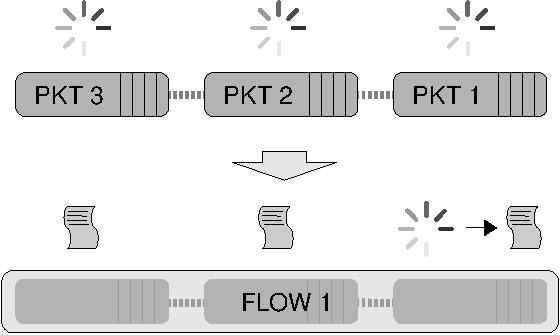
\includegraphics[scale=0.45]{figures/packet_vs_flow-crop} 
    &
    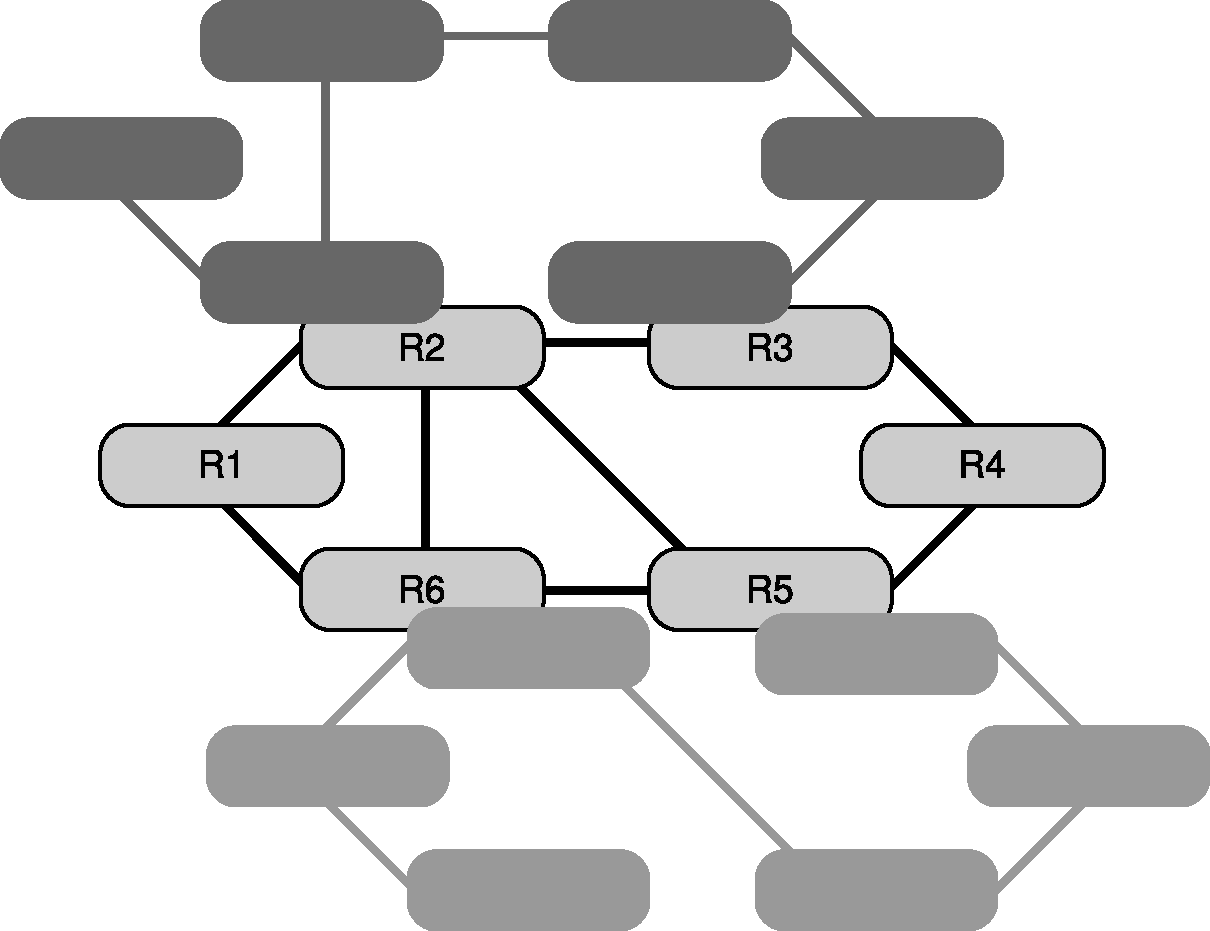
\includegraphics[scale=0.2]{figures/network_virtualization_2}
    \\
    \tiny Agregacion de flujos
    &
    \tiny Virtualizacion de redes
    \\
  \end{tabularx}


\end{frame}  
  
   
\begin {frame}{Tecnologías Actuales}   
  
  Requerimientos $\rightarrow$ {\bf flexibilidad, performance} 
  
  \begin{block}<+->{Circuitos de Propósito Específico (ASICs)} 
    \begin{itemize}
      \scriptsize
      \item Cientos de bloques especializados trabajando en paralelo
      \item Alto desempeño. No programables, alto costo y tiempo de desarrollo.
    \end{itemize}
  \end{block}

  \begin{block}<+->{Network Processors (NPs)}   
    \begin{itemize}
      \scriptsize
      \item Múltiples elementos de procesamiento, buena performance para ciertas tareas. IXP(Intel), PowerNP (IBM)
      \item Difícil portabilidad, interfaces propietarias
    \end{itemize}
  \end{block}

  \begin{block}<+->{Procesadores de Propósito General (GPPs)} 
    \begin{itemize}
      \scriptsize
      \item Arquitectura PC + Software especializado: \emph{Click}, \emph{Zebra/Xorp/Quagga}
      \item Alta flexibilidad, bajo costo. Limitación por transacciones con RAM y naturaleza secuencial
    \end{itemize}
  \end{block}
  
\end{frame}


\begin{frame}{Nuevas tecnologías}

  \begin{block}<+->{Dispositivos Lógicos Programables (FPGAs)} 
    \begin{itemize}
      \scriptsize
      \item Permiten \emph{reconfiguración} y \emph{reprogramación}, contando con librerías de \emph{Open Hardware}. 
      \item Su performance no es lejana a la de un ASIC. Fabricantes: Altera, Xilinx, Actel.
      \item Incorporación creciente de bloques \emph{hardcore} especializados
    \end{itemize}      
  \end{block}
    \vskip3ex
    \center 
    \newcolumntype{V}{>{\centering\arraybackslash} m{.3\linewidth} }
    \begin{tabularx}{\linewidth}{VVV}
      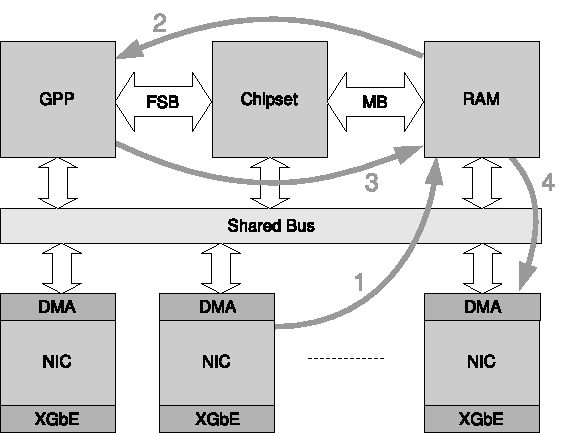
\includegraphics[scale=0.35]{figures/GPP_based}
      &
      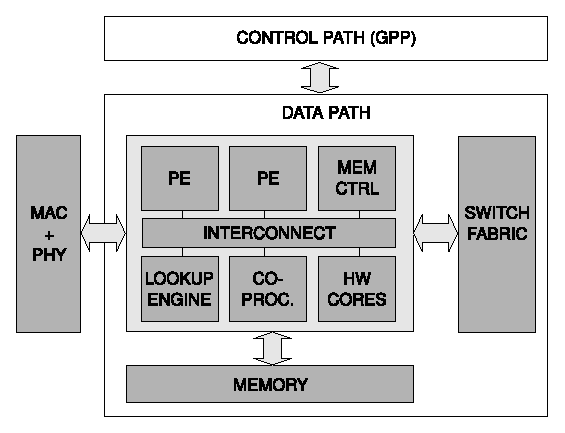
\includegraphics[scale=0.35]{figures/NP_based}
      &
      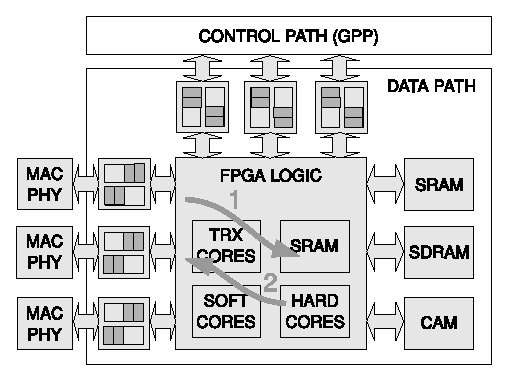
\includegraphics[scale=0.38]{figures/FPGA_based}
      \\
      \tiny Implementación con GPPs
      &
      \tiny Implementación con NPs
      &
      \tiny Implementación con FPGAs
      \\
    \end{tabularx}
\end{frame}

\subsection{Investigación y Desarrollo}
\begin{frame}{Investigación y Desarrollo}
  \begin{block}<+->{Tendencias actuales} 
    \begin{itemize}
      \item Arquitecturas {\bf reconfigurables} y {\bf reprogramables} para adaptarse a nuevas aplicaciones
      \item Arquitecturas {\bf eficientes} para satisfacer exigencias de consumo y velocidad
      \item Extensión del \emph{Open Software} mediante \emph{Open Hardware}
      \item {\bf Métricas a evaluar:} paralelismo vs. consumo de memoria/lógica, velocidad
    \end{itemize}
      
%      \vskip1cm
     \center
     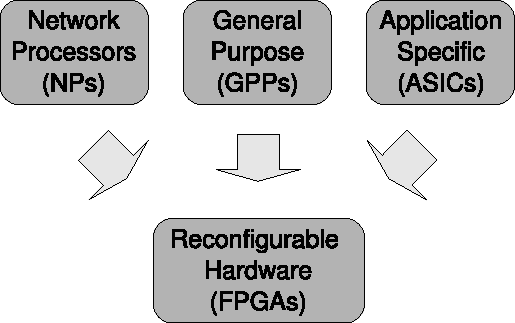
\includegraphics[scale=0.4]{figures/implementation}
  \end{block}
  
  
  \begin{block}<+->{Propuestas}  
    \begin{itemize}
      \item Procesamiento de {\bf flujos} de paquetes en arquitecturas {\bf reconfigurables}
      \item Desarrollo de implementaciones {\bf a medida} de la aplicación
      \item Integración en arquitecturas de procesamiento \emph{asistido por hardware}
    \end{itemize}
  \end{block}

\end{frame}


\begin{frame}{Trabajos Relacionados}
  \begin{block}<1->{Click Modular Router (MIT)}
    \begin{itemize}
    \scriptsize
      \item Librería de objetos {\bf Software} libre, conectados mediante lenguaje propio
      \item Ejecutable a nivel de \emph{usuario} o de \emph{kernel}
      \item Sufre limitaciones por su naturaleza secuencial 
      \item Migración automática a hardware $\rightarrow$ difícil de lograr
    \end{itemize}
 
%    \center
%    \includegraphics[scale=0.3]{figures/click}

  \end{block}

  \pause

  \begin{block}<2->{NetFPGA (Stanford)}
    \begin{itemize}
    \scriptsize
     \item Plataforma {\bf Hardware} basada en un FPGA Xilinx Virtex 5
     \item Versión 10 GbE liberada en 2010
     \item Sistema base \emph{predefinido} para \emph{incorporación} de funcionalidades
    \end{itemize}
    \begin{center}
      \includegraphics<2->[scale=0.2]{figures/netfpga}
    \end{center}
  \end{block}  
\end{frame}

%\begin{frame}{Nuevas tecnologías (3)}
%\begin{itemize}
%\item {\bf Ejemplo 2:} Proyecto NetFPGA - Xilinx Virtex-5 (Xilinx)
%  \begin{itemize}
%    \scriptsize
%    \item hasta 37.440 slices (4 LUTs, 4 FFs)
%    \item hasta 16 Mbits BRAM
%    \item Soporta 4x10 GbE / 1 GbE interfaces
%    \item X8 PCI Express Gen 2 (5Gbps/lane)
%    \item 20 Configurable GTX Serial Transceivers 
%    \item Tres x36 QDR II ( CY7C1515JV18)
%    \item Cuatro x32 RLDRAM II ( MT49H16M36HT-25)
%  \end{itemize}
%\end{itemize}

%  \center
%  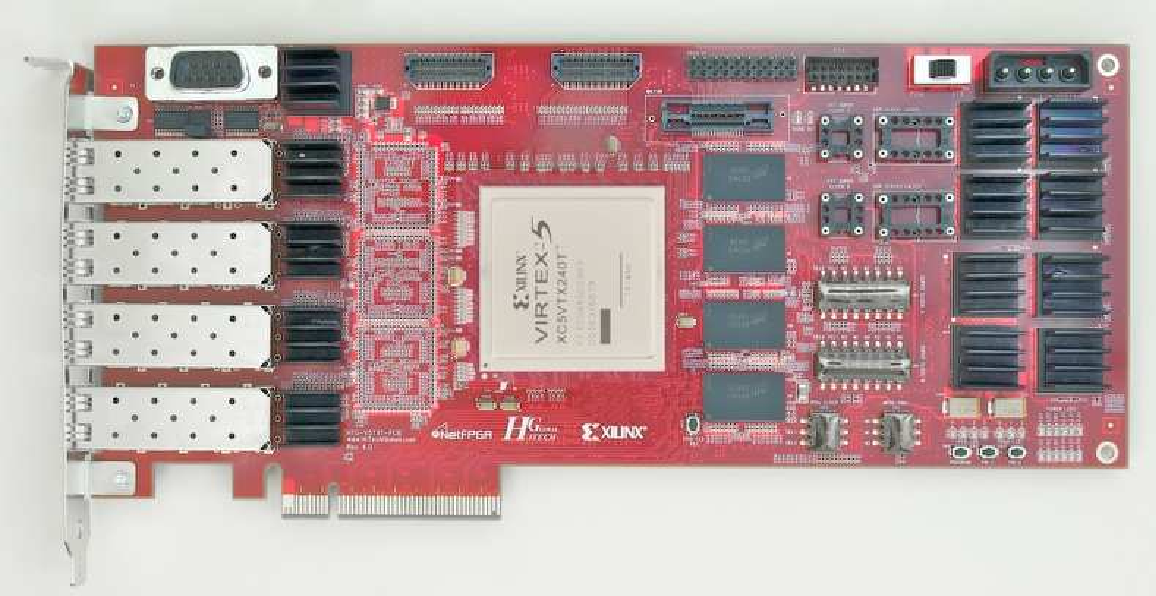
\includegraphics[scale=0.3]{figures/netfpga}

%\end{frame}

\section{Procesamiento en Redes}
\subsection{Introduccion}
\begin{frame}{Procesamiento en Redes}
  \begin{block}<+->{Introducción}
    \begin{itemize}
      \scriptsize
      \item {\bf Básico:} Routing $\rightarrow$ lookup, forwarding, queueing
      \item {\bf Avanzado:} agregación de paquetes, modificación del \emph{camino de datos}
      \item {\bf Caminos de procesamiento}
        \begin{itemize}
        \tiny
          \item \emph{Fast Data Path:} operaciones a velocidad de línea
          \item \emph{Slow Data Path:} operaciones menos frecuentes
        \end{itemize}
      \item {\bf Bloques de interés:} Clasificación, Almacenamiento, Conmutación, Planificación
    \end{itemize}

    \center  
    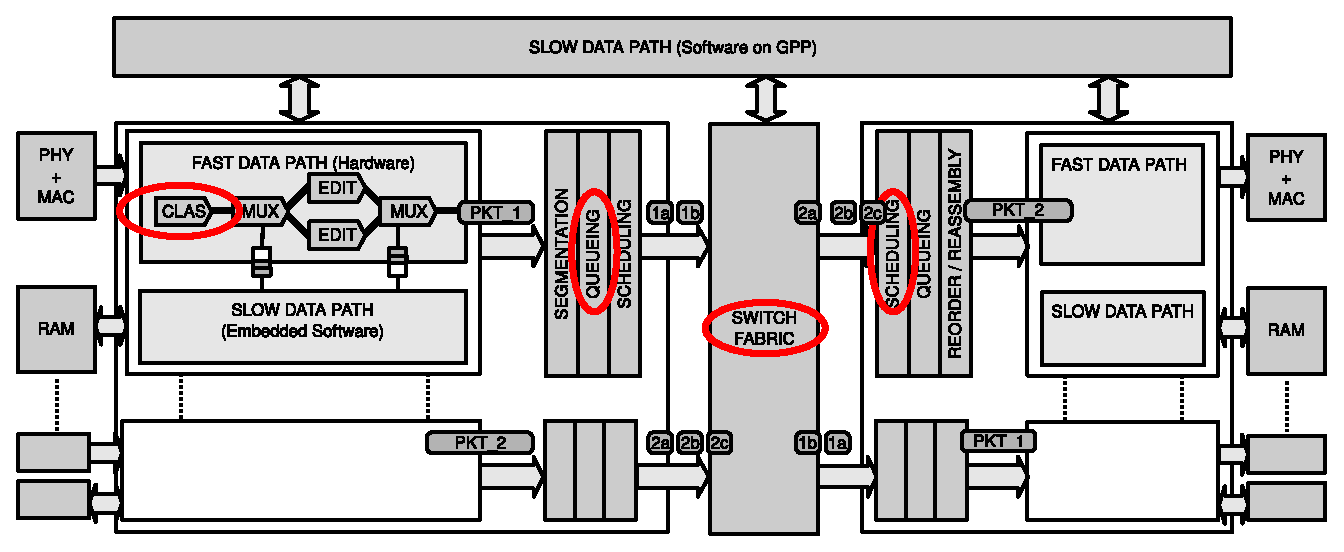
\includegraphics[scale=0.45]{figures/generic_router}
  \end{block}  
  

\end{frame}

\subsection{Clasificación}
\begin{frame}{Procesamiento en Redes de Datos}
  \begin{block}<+->{Clasificación}
    \begin{itemize}
      \item Bloques {\bf esenciales} para procesamiento de flujos diferenciados
      \item Exigencias particulares de \emph{almacenamiento} y \emph{velocidad}
      \item Extracción \emph{configurable} de encabezados contra \emph{uno} o \emph{múltiples} campos $emph$ storage/rule
      \item Matching \emph{exacto} (Protocolo, puertos, MAC) o \emph{mejor} matching (LPM, prefijos IP)
      \item Enfoques de diseño: \emph{algorítmico} (Trees/decomp.) y \emph{arquitectura} (TCAM)
    \end{itemize}
  \end{block}
  
	\begin{columns}
		\begin{column}{0.3\textwidth}
%              \align left
      \center
      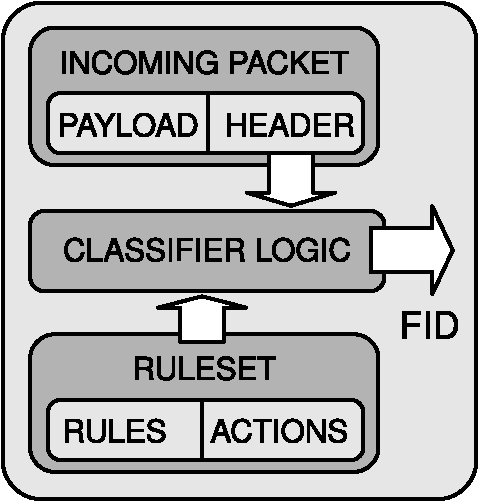
\includegraphics[scale=0.35]{figures/clas_diagram}
      \hskip1cm
%      \tiny Concepto
    \end{column}
    \begin{column}{0.7\textwidth}
      \begin{table}
%      \caption{Implementation of classification}
      \label{classification_table}
      \centering
      \tiny
      \begin{tabular}{ p{2cm} @{\hspace{.5cm}} p{2cm} @{\hspace{.5cm}} p{2cm}} 
      %\begin{tabular}{ p{.315\linewidth} p{.315\linewidth} p{.315\linewidth}} 
      \hline\noalign{\smallskip}
      GPPs        & FPGAs         & ASICs \\
      \noalign{\smallskip}
      \hline
      \noalign{\smallskip} 
      Many rules supported in large and slow SDRAM  & Dedicated registers; low-latency limited internal SRAM; medium-latency external SDRAM & Limited ad-hoc    internal memory; external SDRAM (if interface included) \\
      \noalign{\smallskip}
      Intensive algorithms at low speed & Parallel architectures at wire speed & Parallel architectures at wire speed \\
      \noalign{\smallskip}
      Fully reprogrammable rules & Fully reprogrammable/ reconfigurable rules & Partially \newline reprogrammable rules \\
      \noalign{\smallskip}
      \hline
      \end{tabular}
      \end{table}      
    \end{column}
  \end{columns}
      
%    \item Procedimiento:
%      \begin{itemize}
%        \scriptsize
%        \item almacenamiento de encabezados
%        \item comparación contra una tabla de \emph{reglas}
%        \item edición de un campo de \emph{control}
%      \end{itemize}
%  \end{itemize}
  
%  \vskip1ex


\end{frame}
 
 
\subsection{Conmutación (Switching)}
\begin{frame}{Procesamiento en Redes de Datos}
  \begin{block}<+->{Conmutación (Switching)}
    \begin{itemize}
      \item Múltiples puertos de E/S $\rightarrow$ {\bf Contención}
%     \item Conmutación de \emph{paquetes} o de \emph{celdas}
      \item {\bf Time-division Switching:} bus o memoria compartidos. Soporta tráfico \emph{agregado}. 
      \item {\bf Space-division Switching:} transferencias \emph{simultáneas}. Limitado por efectos \emph{físicos} y \emph{bloqueo interno}.
    \end{itemize}
  \end{block}
  \vskip1ex  
  
	\begin{columns}
		\begin{column}{0.3\textwidth}
      \center
      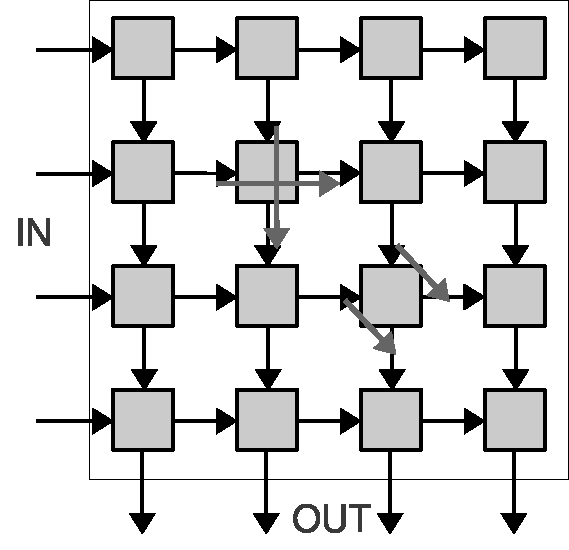
\includegraphics[scale=0.35]{figures/crossbar}
      \hskip1cm
    \end{column}
    
    \begin{column}{0.7\textwidth}
      \begin{table}
%      \caption{Implementation of switching}
        \label{switching_table}
        \centering
        \tiny
        \begin{tabular}{ p{2cm} @{\hspace{.5cm}} p{2cm} @{\hspace{.5cm}} p{2cm}} 
          %\begin{tabular}{ p{.315\linewidth} p{.315\linewidth} p{.315\linewidth}} 
          \hline\noalign{\smallskip}
          GPPs        & FPGAs         & ASICs \\ 
          \noalign{\smallskip}
          \hline
          \noalign{\smallskip}
          Shared bus/memory & Time/space division & Time/space division \\
          \noalign{\smallskip}
          Low/medium \newline performance & High performance & Very high performance \\
          \noalign{\smallskip}
          Little/no optimization possible & Optimization limited by device family & Optimization at design time \\  
          \noalign{\smallskip}
          \hline
        \end{tabular}
      \end{table}
    \end{column}
  \end{columns}
  
\end{frame}  


\subsection{Almacenamiento (Queueing)}
\begin{frame}{Procesamiento en Redes de Datos}
 
  \begin{block}<+->{Almacenamiento (Queueing)}  
    \begin{itemize}
      \scriptsize
      \item Junto con la \emph{Conmutación}, determina desempeño y campo de aplicación
      \item Los buffers absorben \emph{contención} y aplican políticas de QoS
      \item Pueden ubicarse en \emph{entrada}, \emph{salida}, \emph{entrada/salida} o \emph{integrada a la matriz de conmutación}
      \item Almacenamiento de \emph{celdas} o \emph{paquetes} $\rightarrow$ {\bf segmentación/reensamblado}
    \end{itemize}
  \end{block}
 
 	\begin{columns}
		\begin{column}{0.3\textwidth}
      \center
      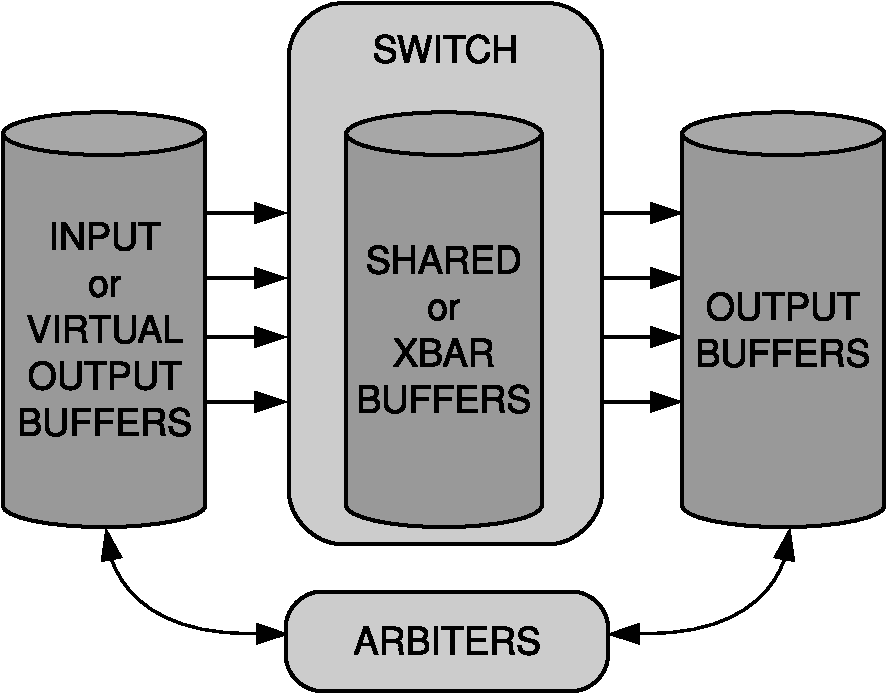
\includegraphics[scale=0.23]{figures/queueing}
      \hskip1cm
    \end{column}
    
    \begin{column}{0.7\textwidth}
      \begin{table}
  %      \caption{Implementation of queueing}
        \label{queueing_table}
        \tiny
        \centering
        \begin{tabular}{ p{2cm} @{\hspace{.4cm}} p{2cm} @{\hspace{.4cm}} p{2cm}} 
        %\begin{tabular}{ p{.315\linewidth} p{.315\linewidth} p{.315\linewidth}} 
        \hline\noalign{\smallskip}
        GPPs        & FPGAs         & ASICs \\ 
        \noalign{\smallskip}
        \hline
        \noalign{\smallskip}
        System SDRAM & Internal SRAM or external SDRAM & Internal SRAM or external SDRAM \\
        \noalign{\smallskip}
        High latency and \newline capacity & Low latency or high \newline capacity & Low latency or High \newline capacity \\
        \noalign{\smallskip}
        Centralized & Centralized/distributed & Centralized \\    
        \noalign{\smallskip}
        \hline
        \end{tabular}
      \end{table}
    \end{column} 
  \end{columns}       
\end{frame}

\subsection{Planificación (scheduling)}
\begin{frame}{Procesamiento en Redes de Datos}
  \begin{block}<+->{Planificación (Scheduling)} 
    \begin{itemize}
      \scriptsize
      \item Surge ante el problema de \emph{contención}
      \item Distribución Equitativa $\rightarrow$ algoritmo \emph{Round-Robin}
      \item Se combina usualmente con el efecto de \emph{policers} (entrada) y \emph{shapers} (salida)
      \item Fuertemente condicionado por la función de \emph{Switching}
    \end{itemize}
  \end{block}
  
  \vskip.5cm
  
  \begin{columns}
		\begin{column}{0.4\textwidth}
      \center
      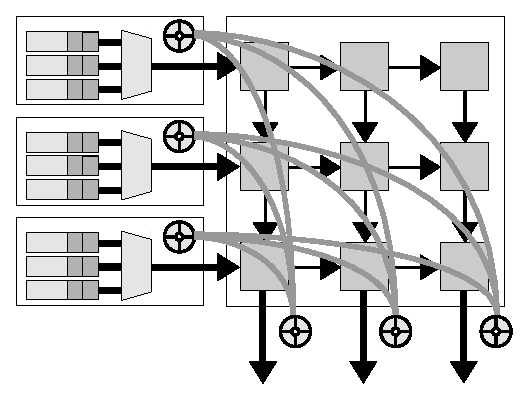
\includegraphics[scale=0.5]{figures/VOQ_scheduling}
      \hskip1cm
    \end{column}
    
    \begin{column}{0.6\textwidth}
      \begin{table}
%      \caption{Implementation of scheduling}
      \label{scheduling_table}
      \centering
      \begin{tabular}{ p{2cm} @{\hspace{.5cm}} p{2cm} @{\hspace{.5cm}} p{1cm}} 
      %\begin{tabular}{ p{.3\linewidth} p{.3\linewidth} p{.3\linewidth}} 
      \hline\noalign{\smallskip}
      GPPs        & FPGAs         & ASICs \\ 
      \noalign{\smallskip}
      \hline
      \noalign{\smallskip}
      Programmable & Configurable/ \newline Programmable & Fixed \\
      \noalign{\smallskip}
      Slow & Medium & Fast \\
      \noalign{\smallskip}
      \hline
      \end{tabular}
      \end{table}
    \end{column} 
  \end{columns}

\end{frame}


\section{Caso de Estudio}
\subsection{Arquitectura planteada}
\begin{frame}{Caso de Estudio}

\begin{block}<+->{Arquitectura planteada} 
  \begin{itemize}
    \scriptsize
    \item {\bf Premisa:} utilizar sólo \emph{lo necesario} en la \emph{ubicación necesaria}
    \item Escenario de aplicación $\rightarrow$ {\bf Conmutación entre LAN Virtuales (VLANs)}
    \item Configuración \emph{Router on a Stick:} múltiples flujos (VLANs) se transportan mediante un \emph{enlace troncal} único
    \item Los puertos de un \emph{Switch} de Capa 2 se agrupan en LANs virtuales. La conmutación \emph{entre VLANs} se realiza en un \emph{Router} de Capa 3 (FPGA)   
  \end{itemize}
\end{block}

\vskip.1cm

  \begin{columns}
    \begin{column}{0.4\textwidth}
      \center
      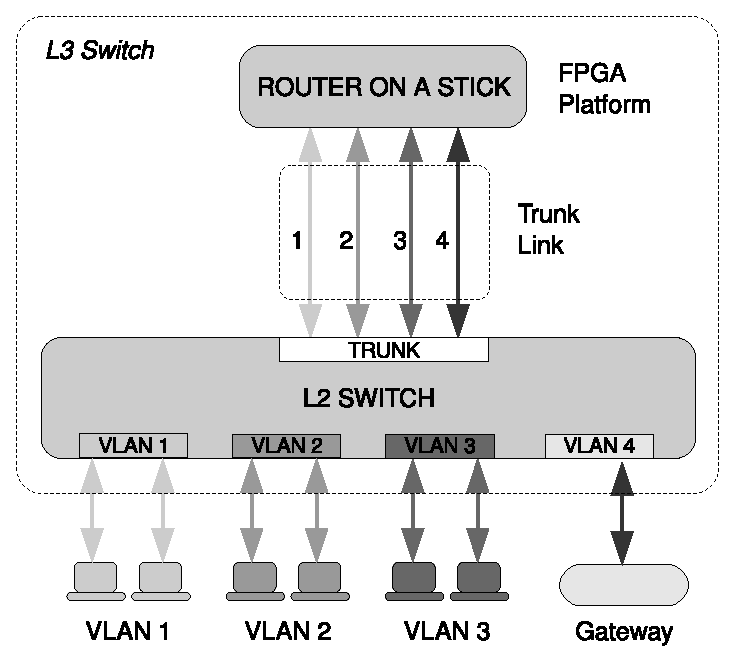
\includegraphics[scale=0.35]{figures/vlan_scenario}
%      \hskip.5cm
    \end{column}
    \begin{column}{0.6\textwidth}
      \center
      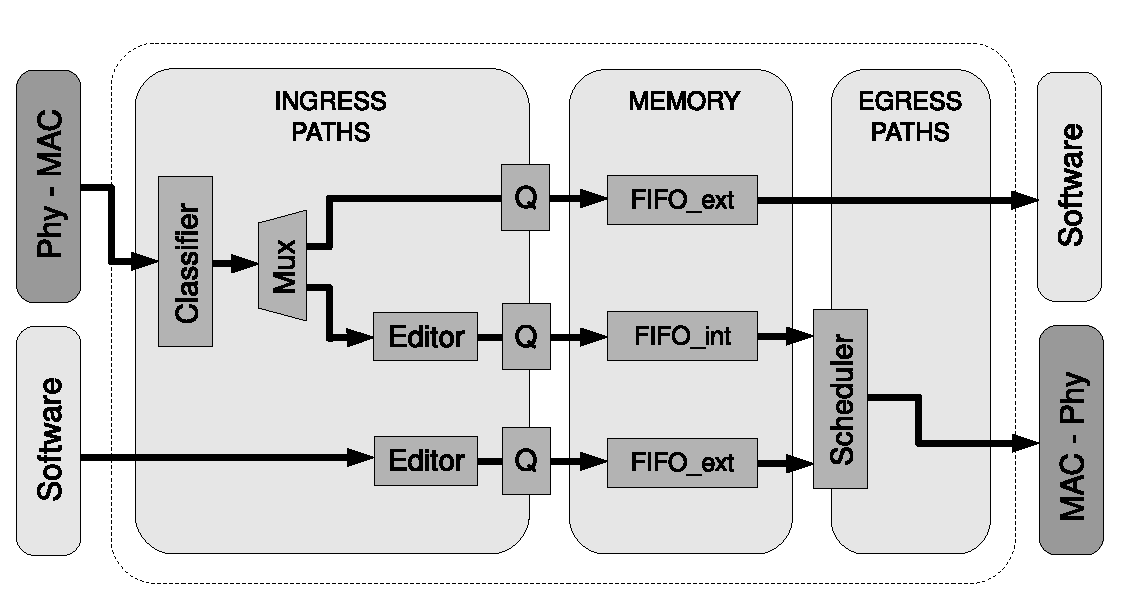
\includegraphics[scale=0.3]{figures/case}
      \hskip6cm

    \end{column}
  \end{columns}

\end{frame}


\subsection{Resultados}
\begin{frame}{Caso de Estudio}

\begin{block}<+->{Resultados}
  \center

  \begin{table}[h]
  \renewcommand{\arraystretch}{1.3}
  %\caption{Resource utilization for case study}
  \label{all}
  \centering
  \tiny
  \begin{tabular}{|c|c|c|} \hline
  Stage & Comb. ALUTs & Registers \\ \hline
  Classifier (8 rules) & 70 & 231  \\
  Queuers (3)  & 179 & 84 \\
  Scheduler  & 180 & 139 \\
  Editors (2) & 77 & 327 \\ \hline
  \emph {Total processing stages} & 506 & 781 \\ \hline
  MAC IP Core and glue logic & 1906 & 1792 \\ \hline
  \emph {Total resources utilization} & 2412 & 2573 \\ \hline
     
  \end{tabular}
  \end{table}

  \begin{columns}
	  \begin{column}{0.4\textwidth}
      \center
      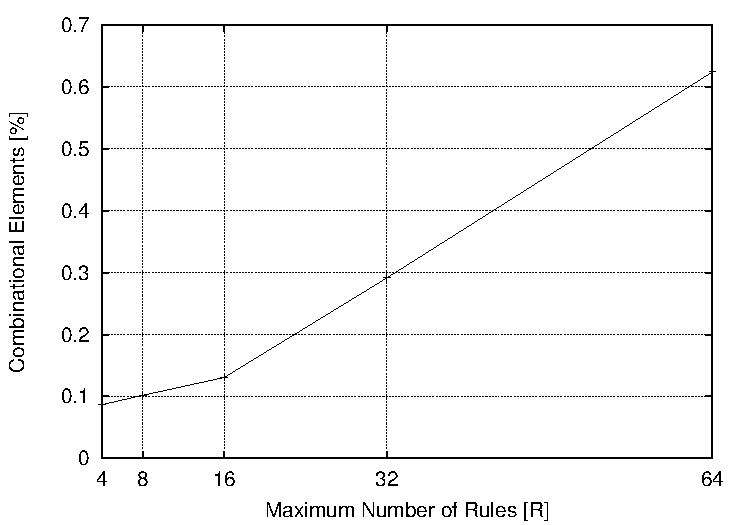
\includegraphics[scale=0.35]{figures/comb}
      \hskip1cm
    \end{column} 
    
    \begin{column}{0.4\textwidth}
      \center
      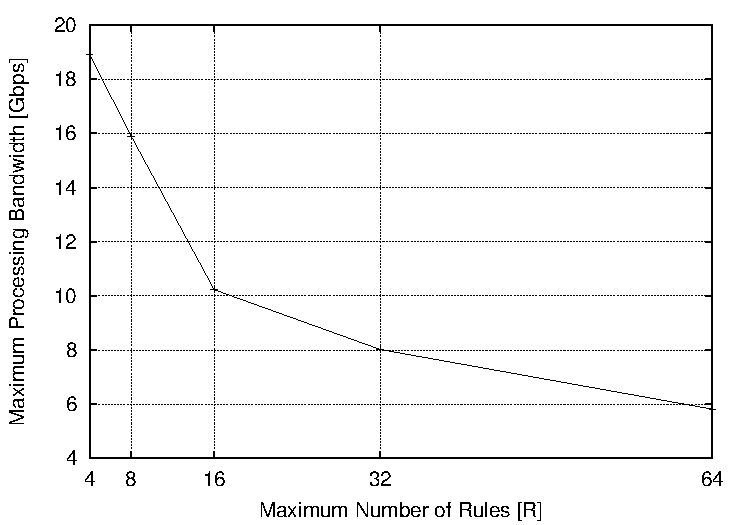
\includegraphics[scale=0.35]{figures/bw}
    \end{column}
  \end{columns}  

\end{block}

%\item La tecnología de lógica programable es muy apropiada para experimentación con arquitecturas distribuidas por su flexibilidad y buen desempeño
%\item Esta tecnología se encuentra en pleno desarrollo
%\item Se investiga la utilización de lenguajes de Alto Nivel (HLLs) para facilitar la programación
%\item Se comprobó que una arquitectura sin optimizaciones fue capaz de implementar un caso medio de uso
%\item Se puede lograr buena escalabilidad incorporando las optimizaciones mencionadas

%\end{itemize}
\end{frame}

\subsection{Conclusiones}
\begin{frame}{Conclusiones}

  \begin{block}<+->{Experiencia realizada}
    \begin{itemize}
      \item La arquitectura conceptual implementada consume menos de 1 \% de recursos en un FPGA \emph{Altera Stratix IIGX}
      \item Trabajo \emph{sin optimizaciones} a velocidad 10 GbE 
      \item Sin embargo, su escalabilidad es limitada $\rightarrow$ campo para {\bf optimizaciones}	
    \end{itemize}
  \end{block}
    
  \begin{block}<+->{Expectativas}
    \begin{itemize}
      \item Contrastación de posibles optimizaciones y evaluación de otros escenarios
      \item Integración con plataforma \emph{software} para migración parcial de funciones 
      \item La evolución de esta tecnología acompañará el trabajo de optimización
      \item {\bf Factor limitante:} largos ciclos de implementación $\rightarrow$ {\bf Lenguajes de Alto Nivel (HLLs)}
    \end{itemize}
  \end{block}
\end{frame}

\begin{frame}{Preguntas}

\huge Gracias por su atención, preguntas?

\vskip3ex

\small jfinochietto@efn.uncor.edu \\
\small czerbini@electronica.frc.utn.edu.ar

\end{frame}


\end{document}

